\documentclass{article}%
\usepackage[T1]{fontenc}%
\usepackage[utf8]{inputenc}%
\usepackage{lmodern}%
\usepackage{textcomp}%
\usepackage{lastpage}%
\usepackage{geometry}%
\geometry{head=40pt,margin=0.8in,bottom=0.8in,includeheadfoot=True}%
\usepackage{xcolor}%
\usepackage{graphicx}%
\usepackage{booktabs}%
\usepackage{array}%
\usepackage{longtable}%
\usepackage{fancyhdr}%
\usepackage{titlesec}%
\usepackage{tcolorbox}%
\usepackage{amsmath}%
\usepackage{enumitem}%
%
\definecolor{titlecolor}{HTML}{2c3e50}%
\definecolor{headercolor}{HTML}{34495e}%
\definecolor{accentcolor}{HTML}{3498db}%
\definecolor{storycolor}{HTML}{27ae60}%
\definecolor{bgcolor}{HTML}{f8f9fa}%

            \titleformat{\section}
              {\Large\bfseries\color{titlecolor}}
              {\thesection}{1em}{}
            \titleformat{\subsection}
              {\large\bfseries\color{headercolor}}
              {\thesubsection}{1em}{}
        %

            \newtcolorbox{storybox}[1][]{
              colback=bgcolor,
              colframe=storycolor,
              coltitle=white,
              fonttitle=\bfseries,
              title=#1,
              rounded corners
            }
            \newtcolorbox{chapterbox}[1][]{
              colback=white,
              colframe=accentcolor,
              coltitle=white,
              fonttitle=\bfseries,
              title=#1,
              rounded corners,
              boxrule=2pt
            }
        %
%
\begin{document}%
\normalsize%
\begin{center}%
\vspace*{2cm}%
{\Huge\bfseries\color{titlecolor} DOUBLE CONICAL SPIRAL}%
\\[0.5cm]%
{\Large\itshape\color{headercolor} Mathematical Perimeter and Physical Net Design}%
\\[2cm]%
\begin{chapterbox}[DESIGN PROCESS]%
\begin{enumerate}[label=Section \arabic*:,leftmargin=2cm]%
\item%
\textbf{Understanding the Spiral Geometry} \\ Configuration parameters and mathematical foundation%
\item%
\textbf{Calculating the True Perimeter} \\ Analytical integration vs numerical approximation%
\item%
\textbf{Discovering the Circular Approximation} \\ From XZ projection to simplified circular regions%
\item%
\textbf{Creating the Annular Net} \\ Transforming geometry into manufacturable nets%
\item%
\textbf{Validation and Results} \\ Comparing all methods and final measurements%
\end{enumerate}%
\end{chapterbox}%
\vfill%
\end{center}%
\newpage%
\section{Understanding the Spiral Geometry}%
\label{sec:UnderstandingtheSpiralGeometry}%
\begin{storybox}[Introduction]%
We start by establishing the mathematical basis for double conical spirals.\newline%
            Each configuration presents distinct geometric challenges, influenced by variations in radius, height, and structural complexity.\newline%
            These parameters will guide the design process throughout.%
\end{storybox}%
\vspace{1cm}%


\begin{table}[h!]%
\caption{Configuration Parameters}%
\begin{center}%
\begin{tabular}{@{}|l|c|c|c|c|c|@{}}%
\toprule%
\midrule%
\textbf{Configuration}&\textbf{Outer R}&\textbf{Inner R}&\textbf{Height}&\textbf{Turns}&\textbf{Struct Lines}\\%
\midrule%
Aligned Spirals&15.00&10.00&12.00&8.00&10.00\\%
\midrule\bottomrule%
%
\end{tabular}%
\end{center}%
\end{table}

%
\vspace{1cm}

%
\newpage%
\section{Calculating the True Perimeter}%
\label{sec:CalculatingtheTruePerimeter}%
\begin{storybox}[The Challenge]%
A critical step in our structural design is calculating the true perimeter of each double conical spiral—
            that is, the actual length of material required to construct each spiral path. This perimeter is not trivial
            to compute due to the complex geometry involving conical tapering, variable radii, and helical motion.

            We apply three distinct methods to approach this problem, each offering a different balance of precision and complexity:

            \begin{itemize}
                \item \textbf{Analytical Method:} Based on the arc length of a 3D parametric curve, we compute the exact integral:
                \[
                    L = \int_0^h \sqrt{\left(\frac{dR}{dz}\right)^2 + \left(R(z) \frac{d\theta}{dz}\right)^2 + 1} \, dz
                \]
                where \( R(z) = R_0 \left(1 - \frac{z}{h} \right) \) defines the spiral's decreasing radius with height, and 
                \( \theta(z) = n z \) captures the angular rotation. This method yields the highest accuracy.

                \item \textbf{Numerical Method:} A discrete sampling approach where the spiral path is broken into thousands of small
                linear segments in 3D space. We compute the Euclidean distance between points:
                \[
                    L \approx \sum_{i=1}^{N-1} \sqrt{ \Delta x_i^2 + \Delta y_i^2 + \Delta z_i^2 }
                \]
                This provides a reliable approximation, especially for visual validation.

                \item \textbf{Circular Approximation:} A simplified model that treats each spiral as a series of flat circular arcs in the XY-plane, 
                ignoring vertical movement. The total length becomes:
                \[
                    L = \sum_{i=1}^{N} 2\pi R_i
                \]
                where \( R_i \) is the instantaneous radius at each step. This is useful for quick estimations but underestimates the actual path length.
            \end{itemize}

            Comparing these approaches not only validates our results but also highlights the geometric impact of vertical travel,
            radius tapering, and angular acceleration on material length.%
\end{storybox}%
\vspace{1cm}%


\begin{table}[h!]%
\caption{Perimeter Calculation Results}%
\begin{center}%
\begin{tabular}{@{}|l|c|c|c|c|c|@{}}%
\toprule%
\midrule%
\textbf{Configuration}&\textbf{Analytical}&\textbf{Numerical}&\textbf{Circular}&\textbf{Struct Lines}&\textbf{Total Length}\\%
\midrule%
Aligned Spirals&630.64&630.57&628.32&120.00&750.64\\%
\midrule\bottomrule%
%
\end{tabular}%
\end{center}%
\end{table}

%
\vspace{1cm}

%
\newpage%
\section{The Circular Approximation}%
\label{sec:TheCircularApproximation}%
{\large\itshape\color{accentcolor} Configuration: Aligned Spirals}%
\\[0.5cm]%
\begin{storybox}[The Breakthrough]%
When we examine the XZ projection of our spiral geometry, what appears as a complex 3D curve 
            reveals itself as a series of concentric circles when viewed from the top.

            This insight allows us to:
            \begin{itemize}
                \item Simplify the 3D spiral into manageable circular sections
                \item Create annular (ring-shaped) regions between inner and outer spirals
                \item Design a flat net pattern that can be manufactured and assembled
            \end{itemize}

            For \textbf{Aligned Spirals}, we identified \textbf{8 circular regions} that approximate
            the original spiral geometry while maintaining structural integrity.

            By applying this simplification: complex 3D mathematics becomes
            straightforward 2D circular geometry, perfect for visualization with a close approximation to the spiral.%
\end{storybox}%
\vspace{1cm}%


\begin{table}[h!]%
\caption{Technical Parameters for Aligned Spirals}%
\begin{center}%
\begin{tabular}{@{}|l|c|@{}}%
\toprule%
\midrule%
\textbf{Parameter}&\textbf{Value}\\%
\midrule%
Target Spacing&0.9 units\\%
Arc Span&30°\\%
Arc Density&10 points\\%
Circular Regions&8 layers\\%
\midrule\bottomrule%
%
\end{tabular}%
\end{center}%
\end{table}

%


\begin{figure}[h!]%
\centering%
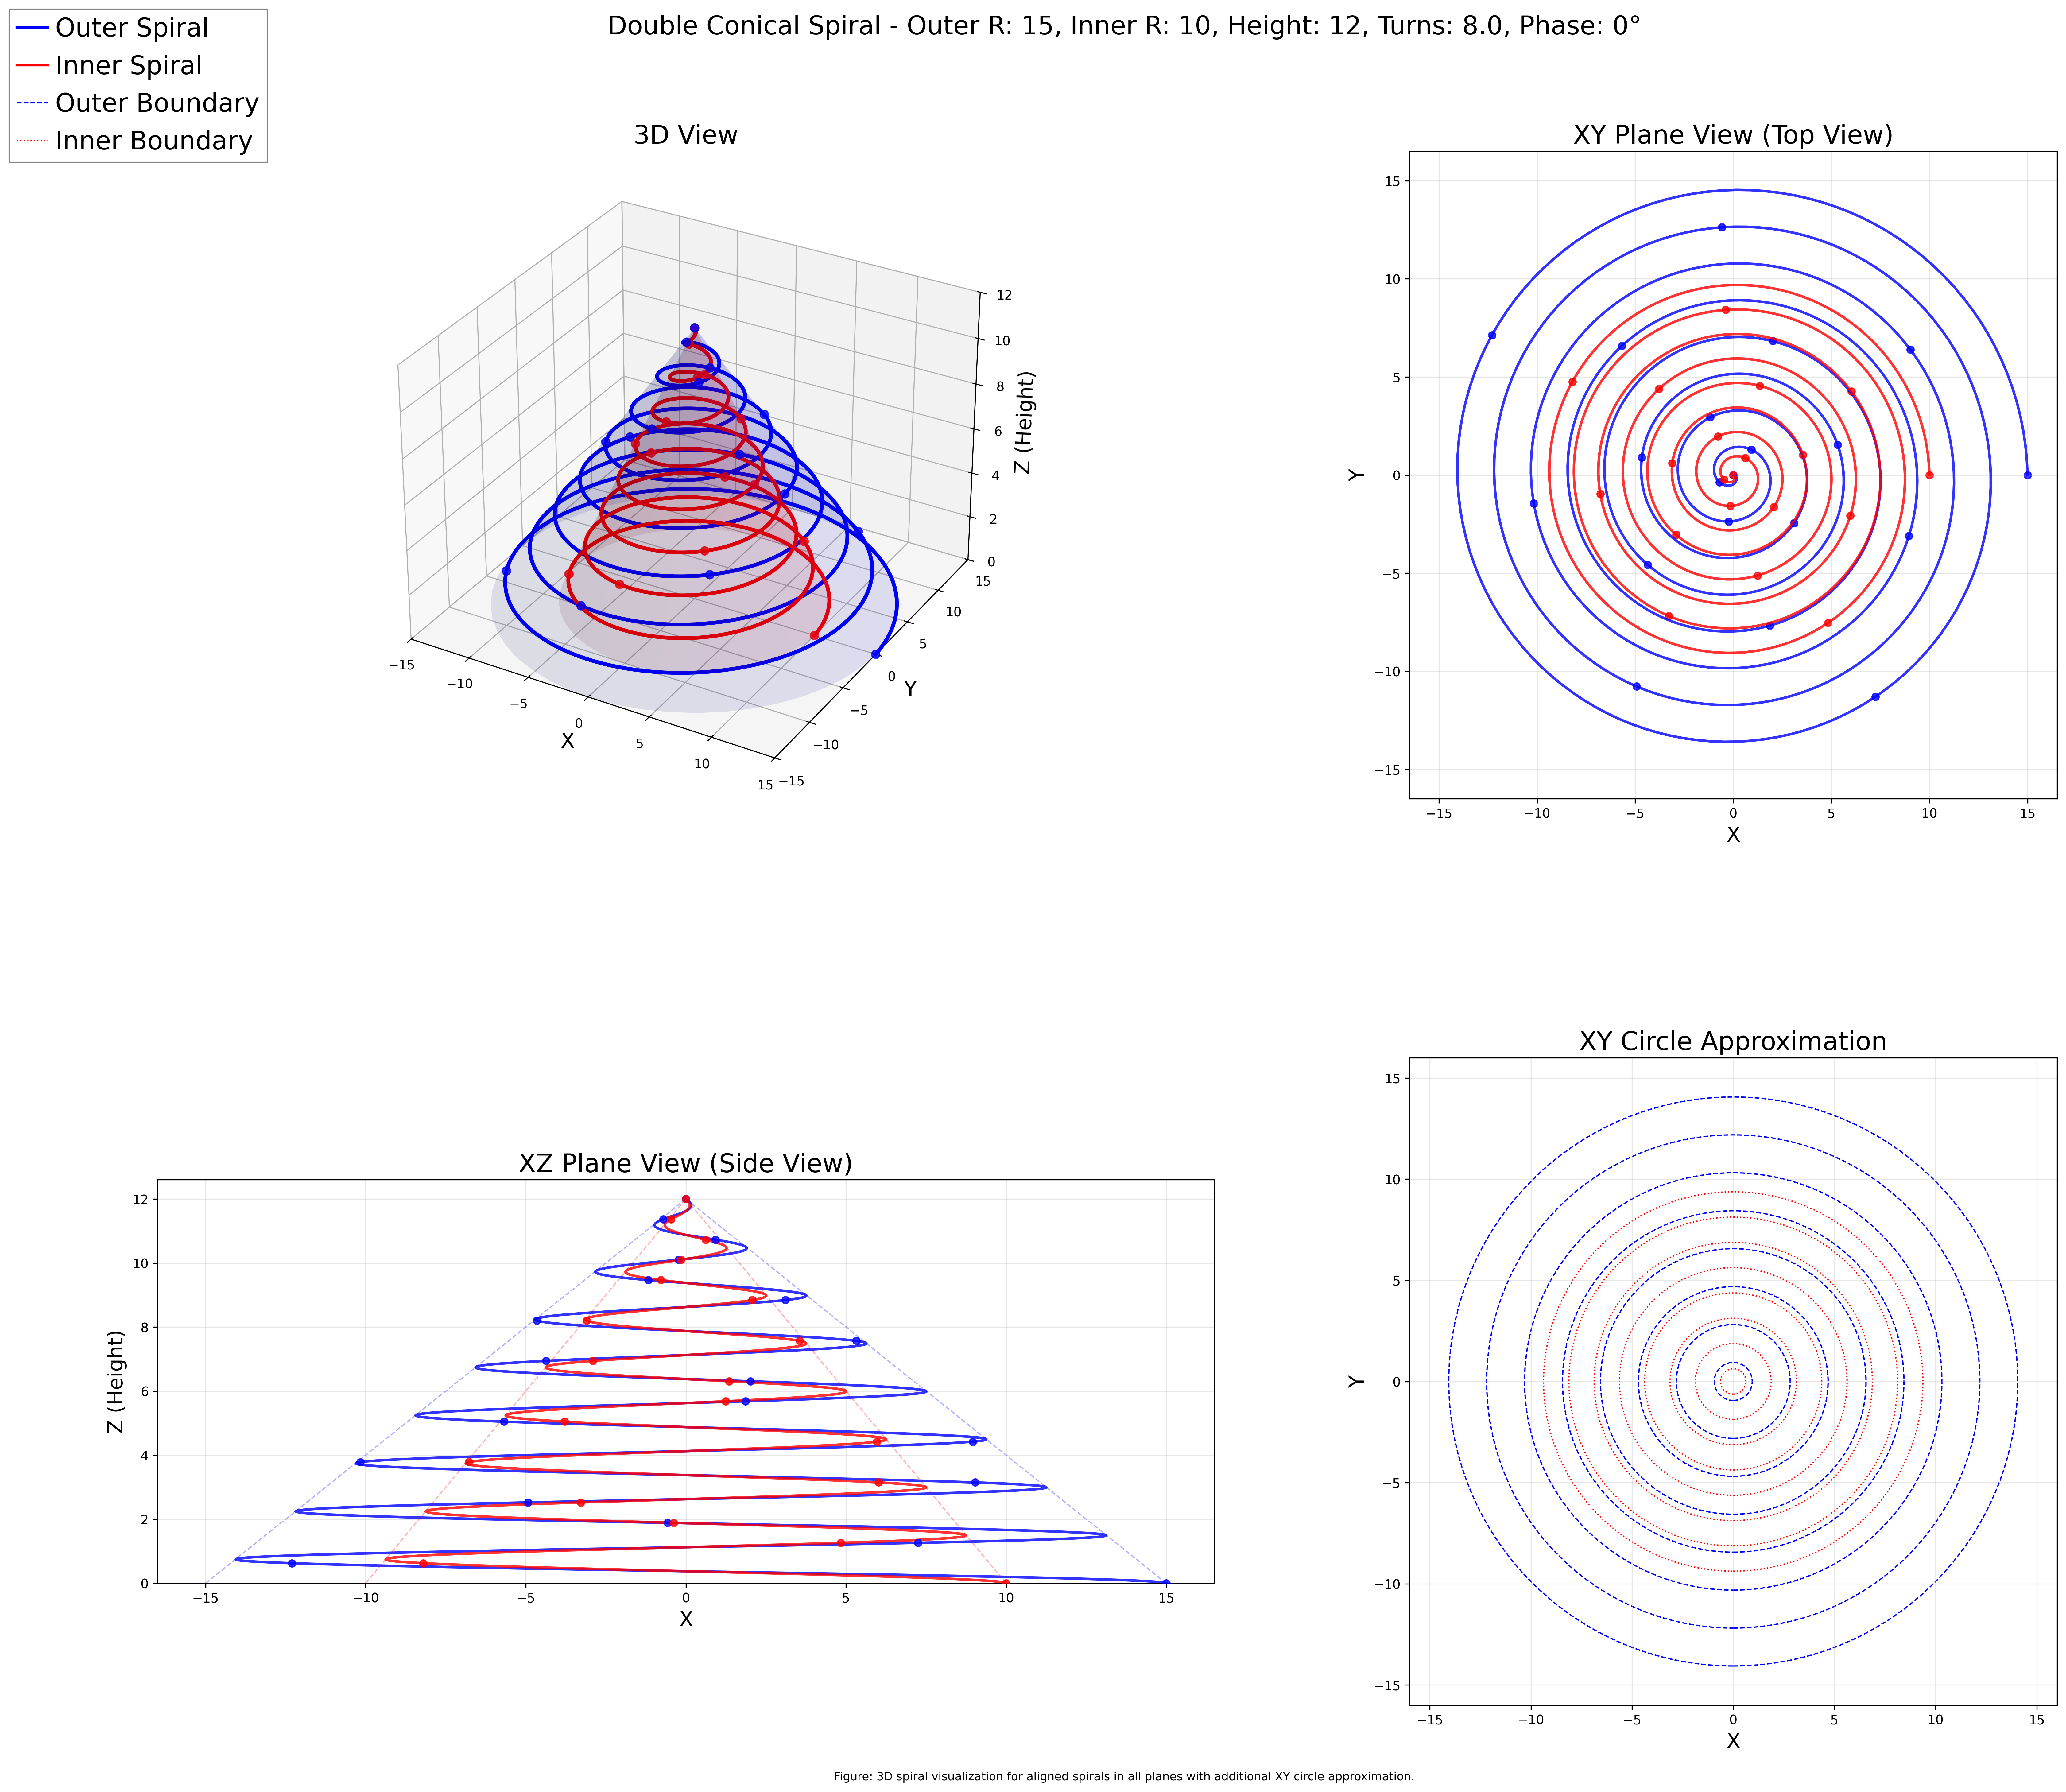
\includegraphics[width=0.8\textwidth]{3d_plot_Aligned_Spirals.png}%
\caption{3D Spiral Geometry {-} Aligned Spirals. Observe the XZ projection (right) showing circular approximation.}%
\end{figure}

%
\vspace{1cm}

%
\newpage%
\section{Creating the Annular Net}%
\label{sec:CreatingtheAnnularNet}%
{\large\itshape\color{accentcolor} Configuration: Aligned Spirals}%
\\[0.5cm]%
\begin{storybox}[The Practical Aproach]%
Now comes the practical aproach: transforming our circular approximation into
            a manufacturable flat pattern -- the annular net.

            \textbf{THE NET CREATION PROCESS:}
            \begin{enumerate}
                \item \textbf{ANNULAR REGIONS:} Each circular layer becomes a ring (annulus) in the flat pattern
                \item \textbf{CONNECTION PATTERN:} We create a web of connections between outer and inner
                    edges within specific angular spans to maintain structural integrity
                \item \textbf{OPTIMIZED SPACING:} Points are distributed to achieve uniform material density
                    with our target spacing of 0.9 units
                \item \textbf{ANGULAR CONTROL:} Each connection spans 30° 
                    with 10 connection points for precision
            \end{enumerate}

            \textbf{RESULT:} The net for Aligned Spirals requires \textbf{12361.41 units} of connecting
            material, creating a pattern that can be cut flat and assembled into the 3D spiral.

            This represents the final step from mathematical concept to physical reality.%
\end{storybox}%


\begin{figure}[h!]%
\centering%
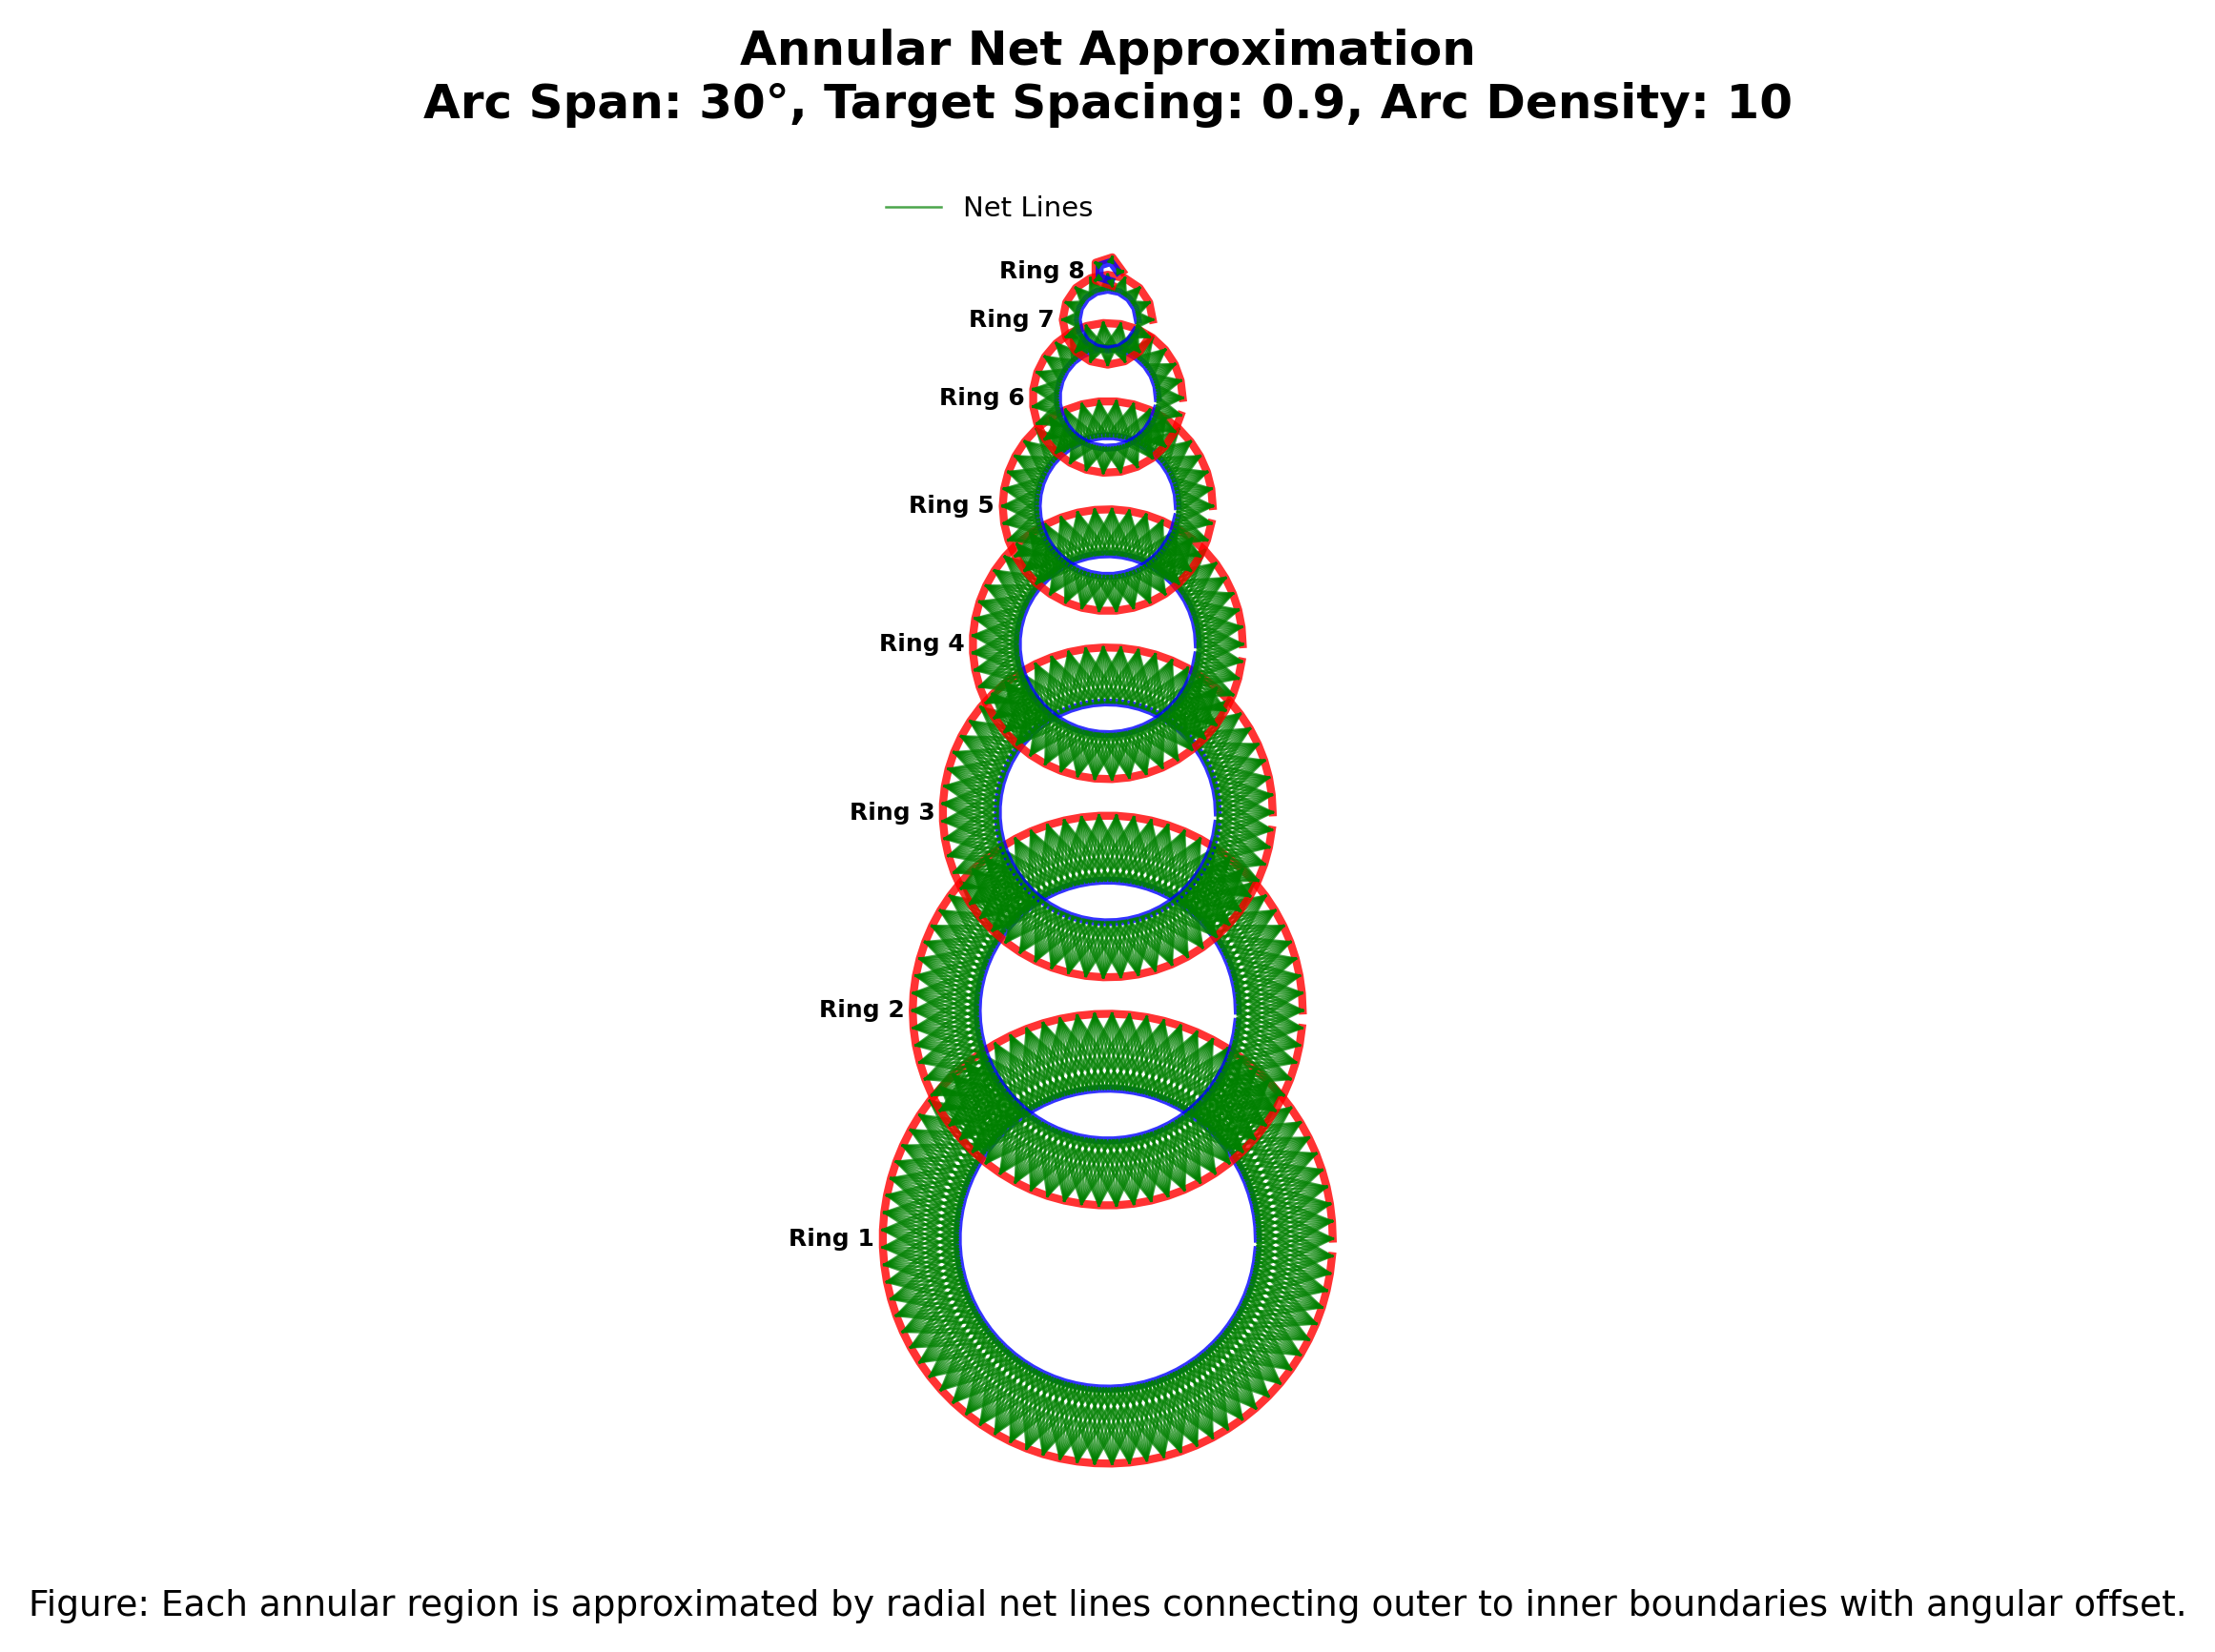
\includegraphics[width=0.8\textwidth]{net_plot_Aligned_Spirals.png}%
\caption{Annular Net Pattern {-} Aligned Spirals. Flat manufacturing pattern for 3D spiral assembly.}%
\end{figure}

%
\vspace{1cm}%
\begin{center}%
{\large\bfseries\color{storycolor} MANUFACTURING READY: 12361.41 units of connecting material in optimized pattern}%
\end{center}

%
\newpage%
\section{Validation and Final Results}%
\label{sec:ValidationandFinalResults}%
\begin{storybox}[Approximation Complete]%
Teh approxiamtion from mathematical spiral to manufacturable net is complete.
            The final validation compares all our methods and confirms the design integrity.

            This comprehensive table shows the complete material requirements for each configuration,
            validating our approach from theoretical calculation through practical implementation.%
\end{storybox}%
\vspace{1cm}%


\begin{table}[h!]%
\caption{Complete Material Requirements Analysis}%
\begin{center}%
\begin{tabular}{@{}|l|c|c|c|c|c|c|@{}}%
\toprule%
\midrule%
\textbf{Config}&\textbf{Analytical}&\textbf{Numerical}&\textbf{Circular}&\textbf{Struct Lines}&\textbf{Net Length}&\textbf{Total Material}\\%
\midrule%
Aligned Spirals&630.64&630.57&628.32&120.00&12361.4120&13112.05\\%
\midrule\bottomrule%
%
\end{tabular}%
\end{center}%
\end{table}

%
\vspace{1cm}%
\begin{storybox}[SUCCESS: Complete Design Validation Achieved!]%
From mathematical perimeter through circular approximation to manufacturable nets,
            this demonstrates how complex 3D geometry can be transformed into
            practical manufacturing solutions while maintaining precision and integrity.

            \textbf{The design is complete.}%
\end{storybox}

%
\end{document}